
\begin{figure}[htbp]
\centering
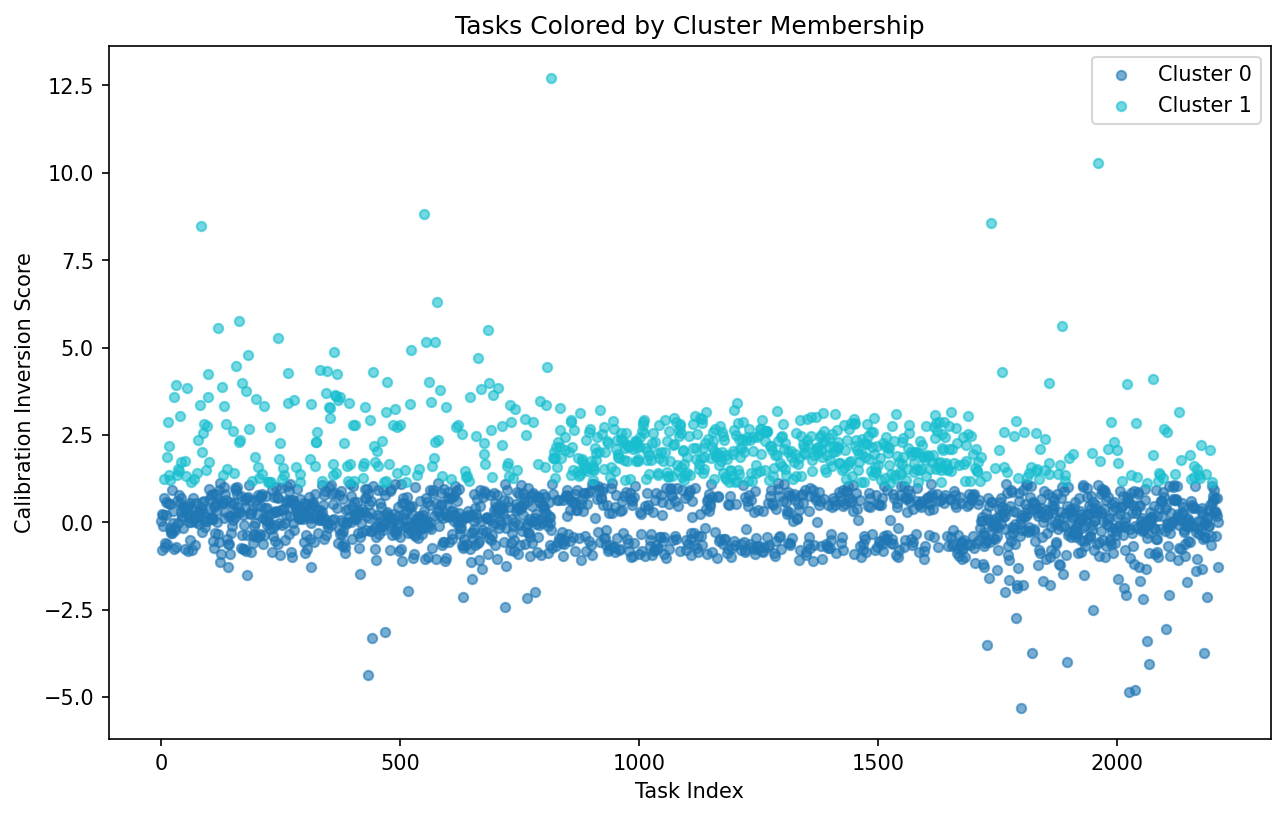
\includegraphics[width=\columnwidth]{figures/cluster_scatter.png}
\caption{Cluster Scatter}
\label{fig:cluster_scatter}
\end{figure}
\textit{Figure 1: Task calibration clustering showing k=2 optimal clusters (silhouette=0.6016). Cluster 0 (1,519 tasks) shows low/no inversion; Cluster 1 (693 tasks) shows high inversion.}

\begin{figure}[htbp]
\centering
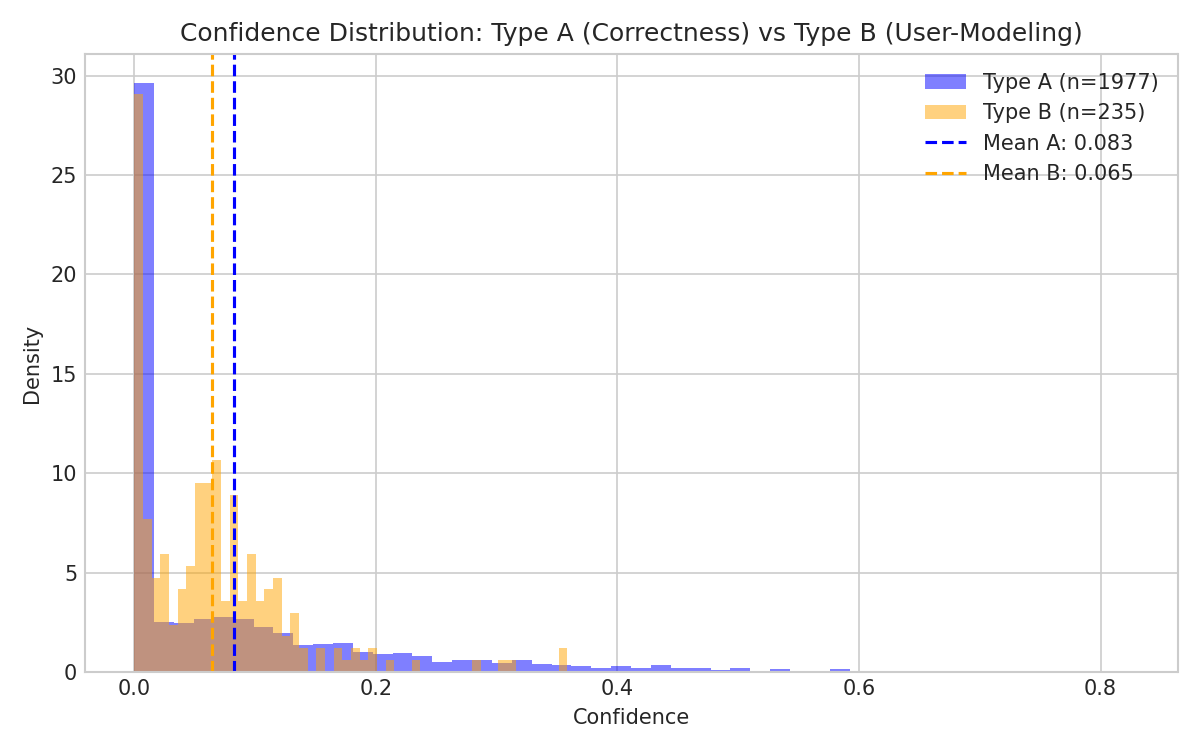
\includegraphics[width=\columnwidth]{figures/confidence_histograms.png}
\caption{Confidence Histograms}
\label{fig:confidence_histograms}
\end{figure}
\textit{Figure 2: Type A vs Type B confidence distributions showing similar patterns across task types (mean\_diff=0.018).}

\begin{figure}[htbp]
\centering
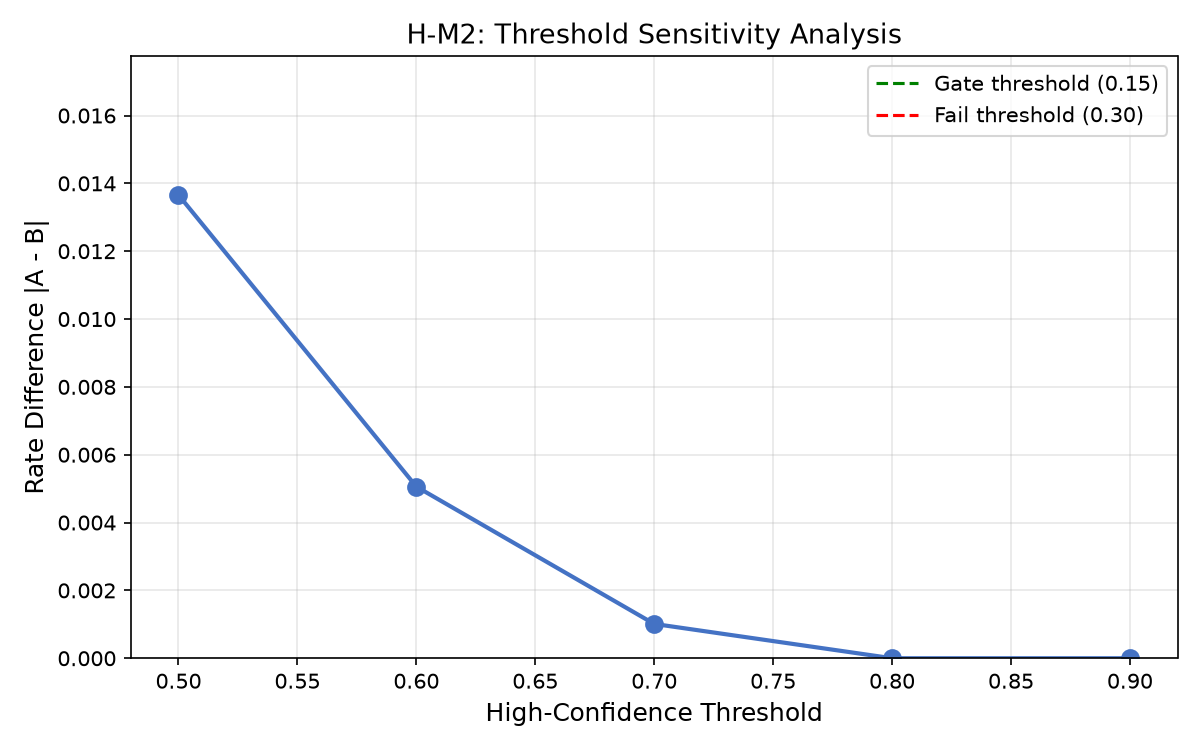
\includegraphics[width=\columnwidth]{figures/sensitivity_curve.png}
\caption{Sensitivity Curve}
\label{fig:sensitivity_curve}
\end{figure}
\textit{Figure 3: Annotator conflation across confidence thresholds. Rate differences remain below 0.02 at all thresholds.}

\begin{figure}[htbp]
\centering
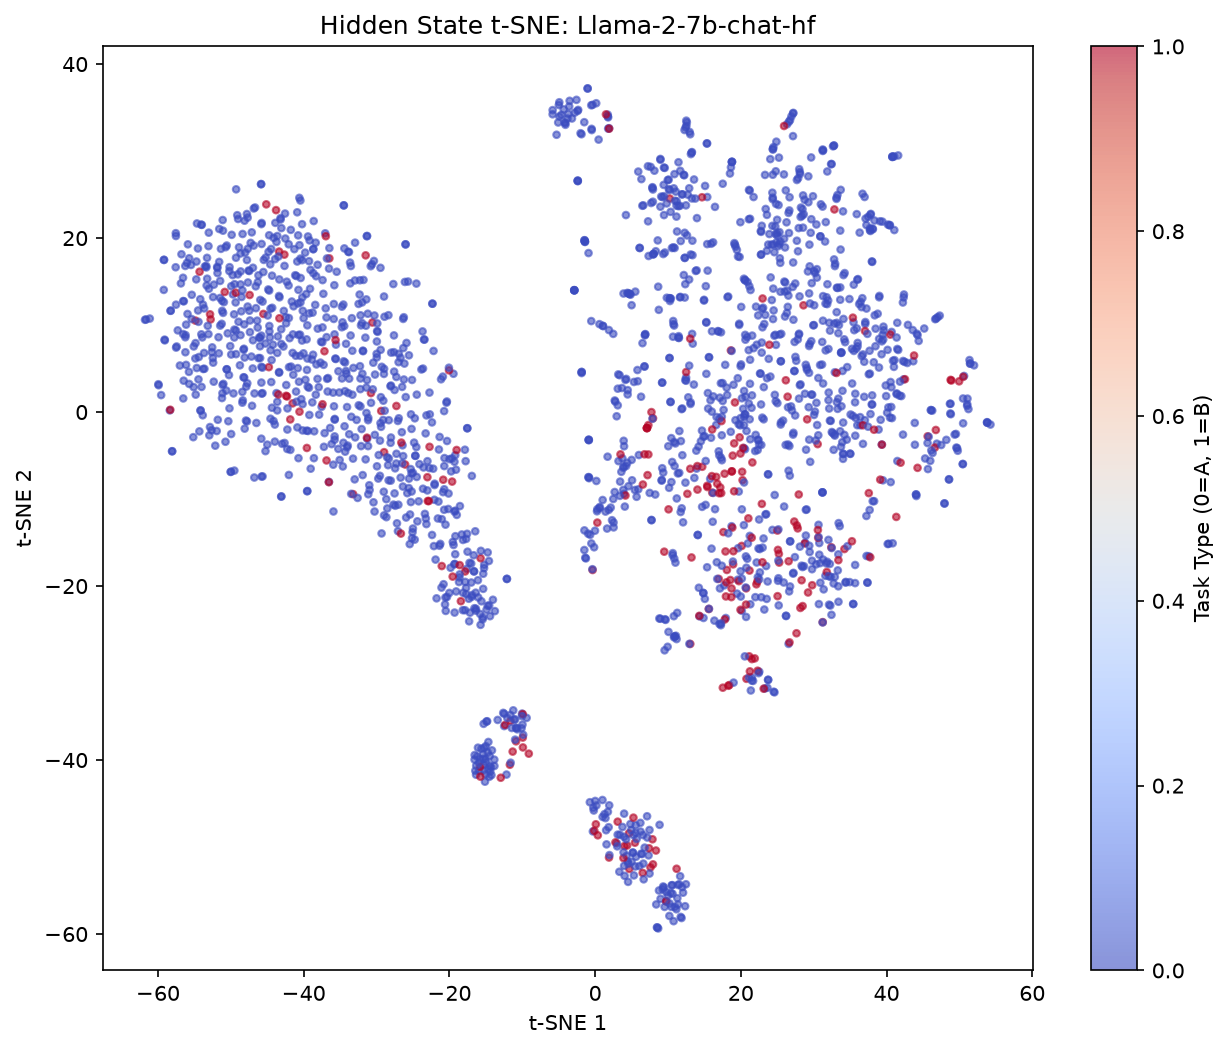
\includegraphics[width=\columnwidth]{figures/tsne_meta-llama_Llama-2-7b-chat-hf.png}
\caption{t-SNE Visualization}
\label{fig:tsne_meta-llama_Llama-2-7b-chat-hf}
\end{figure}
\textit{Figure 4: Hidden state t-SNE visualization showing weak task-type separation (separation=0.024).}

\begin{figure}[htbp]
\centering
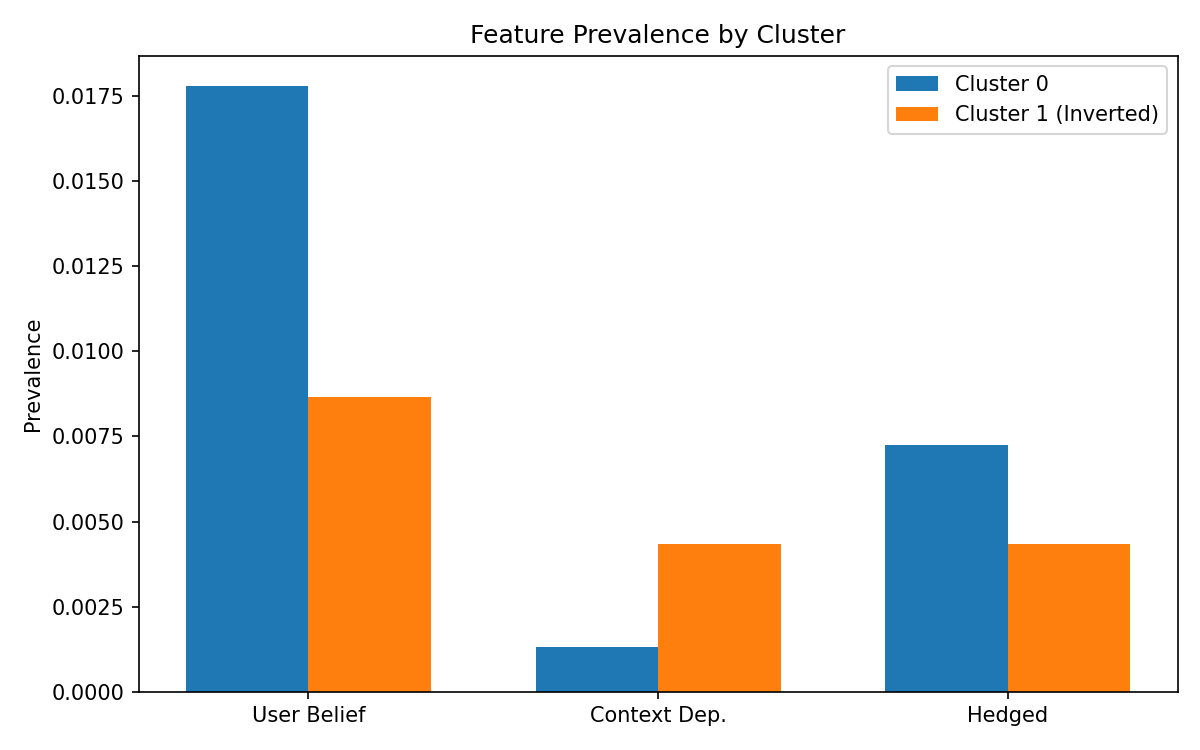
\includegraphics[width=\columnwidth]{figures/feature_breakdown.png}
\caption{Feature Breakdown}
\label{fig:feature_breakdown}
\end{figure}
\textit{Figure 5: Bidirectional feature prevalence by cluster. Total prevalence: 2.3\%.}

\begin{figure}[htbp]
\centering
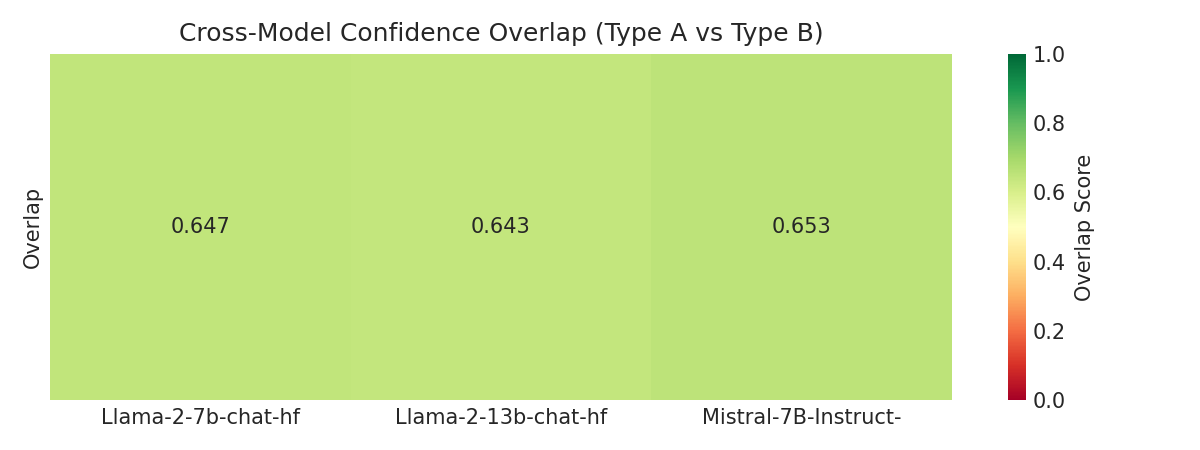
\includegraphics[width=\columnwidth]{figures/cross_model_heatmap.png}
\caption{Cross-Model Heatmap}
\label{fig:cross_model_heatmap}
\end{figure}
\textit{Figure 6: Cross-model overlap scores showing consistent conflation pattern (0.64-0.65 across all models).}
